\documentclass[tikz,border=12pt]{standalone}
\usepackage{sansmath}
\usepackage{amsmath}
\usetikzlibrary{calc}
\sansmath
\renewcommand{\familydefault}{\sfdefault}

\begin{document}
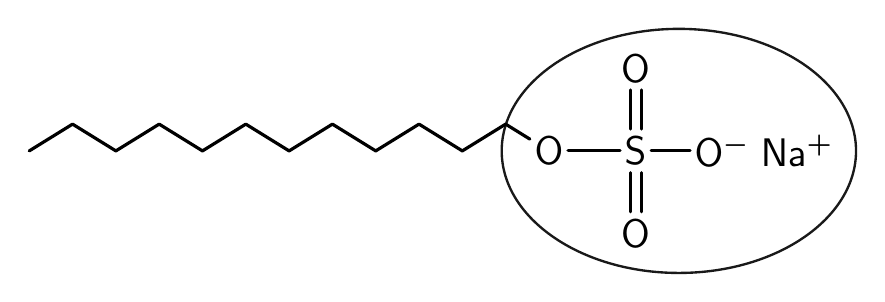
\begin{tikzpicture}[x=1cm, y=1cm, line cap=round, line join=round]
  \tikzset{
    bond/.style={line width=1.15pt, draw=black},
    dbond/.style={line width=1.05pt, draw=black},
    atom/.style={inner sep=1.5pt, font=\sffamily\fontsize{14pt}{16pt}\selectfont}
  }

  % Central Sulfur
  \coordinate (S_pos) at (0, 0);
  \node[atom] (S) at (S_pos) {S};

  % Left Oxygen O1
  \coordinate (O1_pos) at (-1.10, 0);
  \node[atom] (O1) at (O1_pos) {O};
  \draw[bond] (O1) -- (S);

  % Top Oxygen
  \coordinate (Otop_pos) at (0, 1.05);
  \node[atom] (Otop) at (Otop_pos) {O};
  \draw[dbond] ($(S.north) + (-0.07, 0.04)$) -- ($(Otop.south) + (-0.07, -0.04)$);
  \draw[dbond] ($(S.north) + (0.07, 0.04)$) -- ($(Otop.south) + (0.07, -0.04)$);

  % Bottom Oxygen
  \coordinate (Obot_pos) at (0, -1.05);
  \node[atom] (Obot) at (Obot_pos) {O};
  \draw[dbond] ($(S.south) + (-0.07, -0.04)$) -- ($(Obot.north) + (-0.07, 0.04)$);
  \draw[dbond] ($(S.south) + (0.07, -0.04)$) -- ($(Obot.north) + (0.07, 0.04)$);

  % Right Oxygen with negative charge O^-
  \coordinate (Oright_pos) at (1.10, 0);
  \node[atom] (Oright) at (Oright_pos) {O$^{\boldsymbol{-}}$};
  \draw[bond] (S) -- (Oright);

  % Sodium cation Na+
  \coordinate (Na_pos) at (2.05, 0);
  \node[atom] (Na) at (Na_pos) {Na$^{\boldsymbol{+}}$};

  % Ellipse enclosing the head group (hydrophilic head)
  \coordinate (head_center) at (0.55, 0);
  \draw[line width=0.85pt, draw=black!90] (head_center) ellipse (2.25cm and 1.55cm);

  % Alkyl chain: 12 carbons (C1 to C12) - Hydrophobic tail
  \def\dx{0.55}
  \def\dy{0.34}

  \coordinate (C12) at ($(O1_pos) + (-\dx, \dy)$);
  \coordinate (C11) at ($(C12) + (-\dx, -\dy)$);
  \coordinate (C10) at ($(C11) + (-\dx, \dy)$);
  \coordinate (C9)  at ($(C10) + (-\dx, -\dy)$);
  \coordinate (C8)  at ($(C9)  + (-\dx, \dy)$);
  \coordinate (C7)  at ($(C8)  + (-\dx, -\dy)$);
  \coordinate (C6)  at ($(C7)  + (-\dx, \dy)$);
  \coordinate (C5)  at ($(C6)  + (-\dx, -\dy)$);
  \coordinate (C4)  at ($(C5)  + (-\dx, \dy)$);
  \coordinate (C3)  at ($(C4)  + (-\dx, -\dy)$);
  \coordinate (C2)  at ($(C3)  + (-\dx, \dy)$);
  \coordinate (C1)  at ($(C2)  + (-\dx, -\dy)$);

  % Draw alkyl chain
  \draw[bond] (C1) -- (C2) -- (C3) -- (C4) -- (C5) -- (C6) -- (C7) -- (C8) -- (C9) -- (C10) -- (C11) -- (C12);
  
  % Bond C12 straight to O1
  \draw[bond] (C12) -- (O1);

\end{tikzpicture}
\end{document}
